\section{Химические соединения и их характеристики: строение, состав, свойство. Простые и сложные соединения. Стехиометрические соотношения, эмпирическая и молекулярная формула соединения. Валентность элементов.}

\textbf{Химическое соединение} --- сложное вещество, состоящее из химически связанных атомов одного или более элементов. \\ 

\textbf{Простыми} называются вещества, состоящие из атомов одного химического элемента. Например, молекулярные кислород \ce{O2}, водород \ce{H2} и т.д. \textit{Атомарные газы} (типа гелия \ce{He}, аргона \ce{Ar}) назвать \textit{соединениями} нельзя.\\

\textbf{Состав} соединения записывается в виде химической формулы: 

\begin{itemize}
	\item \textit{эмпирическая (простейшая) формула} описывает только соотношение количества элементов в молекуле. Для бензола, например, это \ce{CH}.
	\item \textit{молекулярная формула} отражает число атомов в молекуле. Для бензола \ce{C6H6}. 
\end{itemize}

\textbf{Структурная формула} показывает взаимное расположение атомов в молекуле.

\begin{figure}[H]
	\centering
	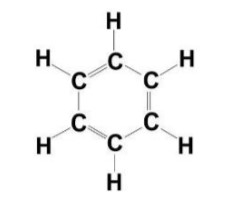
\includegraphics{Pictures/Benzol.jpg}
	\caption{Структурная формула бензола.}
\end{figure}

Соединения характеризуются \textbf{химическими свойствами}: 
\begin{itemize}
	\item способностями реагировать с другими веществами; 
	\item способностью к разложению (реакции, в которой из одного, более
сложного вещества образуется 2 и более других, более простых);
	\item диссоциации (процессу распада на ионы при растворении в воде или плавлении вещества).\\
\end{itemize}

\textit{Молекула} --- электронейтральная частица, состоящая из двух или более атомов.\\

\textbf{Валентность} --- число химических связей, которыми данный атом в молекуле связан с другими. \textit{Для веществ ионного строения:} валентность --- максимальное число одновалентных атомов (например, водорода), которые могут соединяться с атомом данного элемента или на которые этот атом может замещаться.

Валентность обозначается римскими цифрами и может принимать значения от одного до восьми. 

\begin{figure}[H]
	\centering
	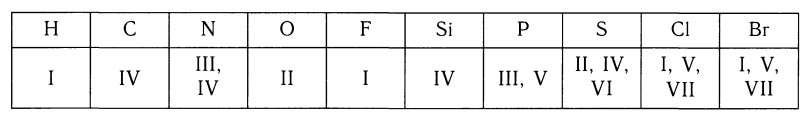
\includegraphics{Pictures/Val.jpg}
	\caption{Характерные валентности некоторых элементов-неметаллов.}
\end{figure}

\textbf{Стехиометрия} --- раздел химии, посвященный расчетам по химическим формулам и уравнениям реакций.\\

\textbf{Основной закон химической стехиометрии:}

\emph{Отношение количеств реагирующих веществ (в молях) равно отношению соответствующих коэффициентов в уравнении реакции.}\\

Например, для реакции \ce{2H2 + O2 -> 2H2O} количества прореагировавших веществ относятся как:

\begin{equation*}
n(\ce{H2}): n(\ce{O2}): n(\ce{H2O}) = 1:2:1.
\end{equation*}
